\subsection{Einf"uhrung in die Monte-Carlo-Methode}

Monte-Carlo-Methoden sind Algorithmen, die Zufallszahlen nutzen um nicht oder nur aufwendig l"osbare Probleme stochastisch zu approximieren. Wie in der Einleitung schon genannt, liefert die Grundlage hierf"ur das starke Gesetz der gro"sen Zahlen.
In diesem Kapitel orientiere ich mich an \cite{MC}.
\begin{sz}[Starkes Gesetz der gro"sen Zahlen]
Sei $(X_i, i\in\mathbb{N})$ eine Folge unabh"angiger, identisch verteilter
Zufallsvariablen in $L^1$. Dann konvergiert die Folge $(S_n, n \in \mathbb{N})$
mit $S_n := \frac{1}{n}\sum_{i=1}^n X_i$ 
fast sicher gegen $\mathbb{E}(X_1).$
\end{sz}
Allgemeines Ziel ist die Approximation einer reellen Zahl $a$. Man konstruiert dann eine reellwertige Zufallsvariable $Y$ mit 
$\mathbb{E}(Y) = a.$\\
$Y$ hei"st \textbf{Basisexperiment} der direkten Simulation.
Man betrachtet anschlie"send eine Folge $(Y_i)_{i\in\mathbb{N}}$ von reellwertigen, unabh"angigen
Zufallsvariablen mit gleicher Verteilung wie Y.
Diese nennt man auch unabh"angige \textbf{Kopien} oder
\textbf{Wiederholungen} von Y.
Die Zahl $a$ wird nun durch $D_n =\frac{1}{n}\sum_{i=1}^n Y_i$ approximiert.
$D_n$ hei"st direkte Simulation oder \textbf{Monte-Carlo-Sch"atzer}.
\begin{sz}\label{var}
F"ur den Fehler der direkten Simulation gilt:
\begin{align*}
\Delta (D_n)=\sqrt{\mathbb{E}(D_n-a)^2}=\sqrt{\frac{Var(Y)}{n}}.
\end{align*}
\end{sz}
\begin{proof}
Es ist 
\begin{align*}
\mathbb{E}(D_n-a)^2= Var(D_n)=Var\left(\frac{1}{n}\sum_{i=^1}^n Y_i\right)=\frac{1}{n^2}Var\left(\sum_{i=^1}^n Y_i\right)\underset{(*)}{=}\frac{1}{n^2}\cdot n\cdot Var(Y)=\frac{Var(Y)}{n}
\end{align*}
$(*)$ da  $Y_i$ unabh"angig 
\end{proof}

\begin{df}[Landau-Symbol]
Gegeben seien zwei reellwertige Funktionen $g,h$. Dann hei"st $g(x)$ von der Ordnung $h(x)$, also $g(x)=\mathcal{O}(h(x))$ falls gilt:
\begin{align*}
\exists C>0 \ \ \exists x_0>0\ \ \forall x>x_0\ : \ |g(x)|\leq C \cdot |h(x)|.
\end{align*}
\end{df}

Mit dieser Definition und obigem Satz gilt also: $Var(D_n)=\mathcal{O}(\frac{1}{n}).$\newpage
\begin{enumerate}
\item \textbf{Die Hit-or-Miss Integration}:\\
Das Ziel ist es eine Funktion $f:[0,1]\rightarrow \mathbb{R}$ zu integrieren.
Bei der Hit-or-Miss Integration macht man direkten Gebrauch von der Interpretation des Integrals als Fl"acheninhalt A.
Wir haben einen Wahrscheinlichkeitsraum $(\Omega,\mathcal{A},\mathbb{P})$ und betrachten die Zufallsvariable $Y=\mathbb{I}_A$.
Die zu untersuchende Fl"ache A wird durch ein Rechteck eingegrenzt und
auf diesem werden mit einer Gleichverteilung zuf"allige Punkte
erzeugt.\\
Es gilt dann $\mathbb{E}(Y ) = \mathbb{P}(A) =\frac{ \text{gesuchter Fl"acheninhalt}}{\text{Fl"ache Rechteck}}$.
Dank dem SGdgZ konvergiert $\frac{\text{Anzahl Treffer}}{\text{Anzahl der Punkte}}$ gegen die Wahrscheinlichkeit $\mathbb{E}(Y)=\mathbb{P}(A)$.
\item \textbf{Direkte Monte-Carlo Integration}:\\
Wiederum ist das Ziel das Integral einer Funktion $f:D\rightarrow \mathbb{R}$ zu approximieren.
Jetzt werden aber aber im Definitionsbereich zuf"allige Werte erzeugt und $f$ wird an diesen Stellen ausgewertet und der Mittelwert dieser Funktionswerte gebildet.
D.h das Integral $S(f) = \int_D f(x) \ \text{dx}$ wird approximiert durch $ M(f) =\frac{1}{n}\sum_{i=1}^n f(X_i)$
mit einer Folge von auf $D$ gleichverteilten,unabh"angigen
Zufallsvektoren $X_i$.
\end{enumerate}

\subsubsection{Beispiel: Berechnung von $\pi$}
In diesem Beispiel wollen wir $\pi$ mit Hilfe des Einheitskreises bzw. eines Einheitskreisviertels berechnen.
Genauer betrachten wir die Menge $G=[0,1]^2$.
\begin{enumerate}
\item[a)]\underline{Die Hit-or-Miss-Methode:}\\
Das Basisexperiment ist die Zufallsvariable $Y := \mathbb{I}_B $ mit \\ 
$B=\{(x_1, x_2) \in G | \  x_1^2+x_2^2\leq1\}$.
Es gilt dann $\mathbb{P}(B) =\mathbb{E}(Y ) =\frac{\pi}{4}$.\\
W"ahlt man nun also zuf"allige Punkte im Einheitsquadrat und bestimmt
den relativen Anteil der Punkte in B, bekommt man eine Approximation
von $\frac{\pi}{4}$. Das bedeutet $4\cdot \frac{\text{Punkte in B}}{\text{Punkte gesamt}}\approx \pi$.
\begin{figure} [H]
\centering
    \subfigure[$n=10^2$]{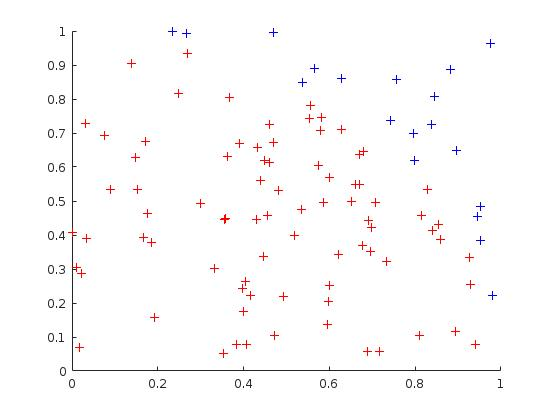
\includegraphics[width=5cm]{10^2.jpg}} 
    \subfigure[$n=10^3$]{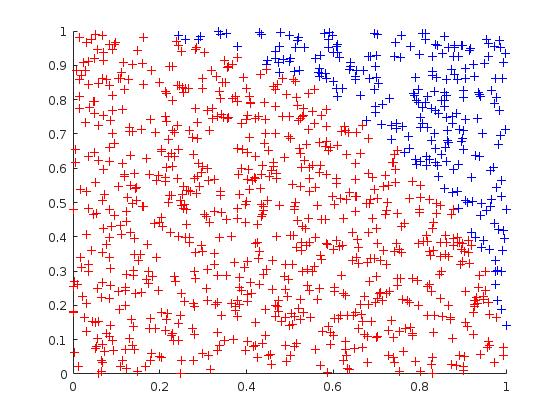
\includegraphics[width=5cm]{10^3.jpg}} 
    \subfigure[$n=10^5$]{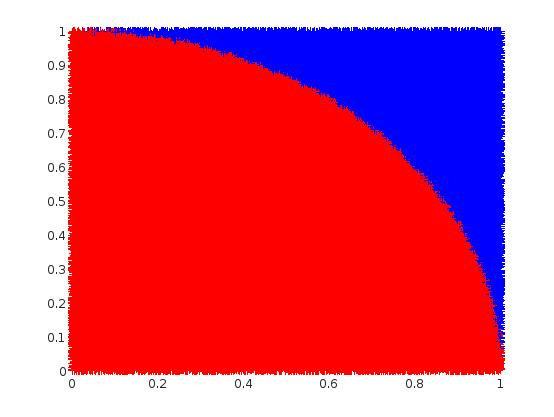
\includegraphics[width=5cm]{10^5.jpg}} 
\end{figure}
\newpage
Die Ergebnisse waren f"ur mehrere Durchl"aufe:
\begin{enumerate}
\item[-]$n=10^2$: $3,24; 3,28; 2,96$
\item[-]$n=10^3$: $3,125; 3,128; 3,104$
\item[-]$n=10^5$: $3,1415; 3,1472; 3,1371$.
\end{enumerate}
\item[b)]\underline{Direkte Simulation:}\\
Wir betrachten die Funktion $g(x)=\sqrt{1-x^2}$. Es seien au"serdem $X_i$ auf $[0,1]$  gleichverteilte unabh"angige Zufallsvariablen. Der Monte-Carlo-Sch"atzer ist dann gegeben durch $D_n:=\frac{1}{n}\sum_{i=1}^n g(X_i)$.

\begin{figure}[H]
\centering
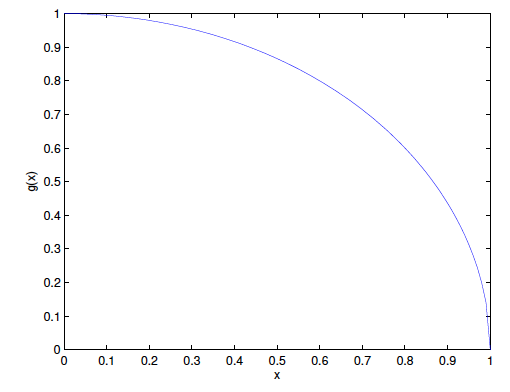
\includegraphics[width=9cm]{Kreis.jpg}
\caption{ Graph der Funktion $g(x)$}
\end{figure}
\begin{figure}[H]
\centering
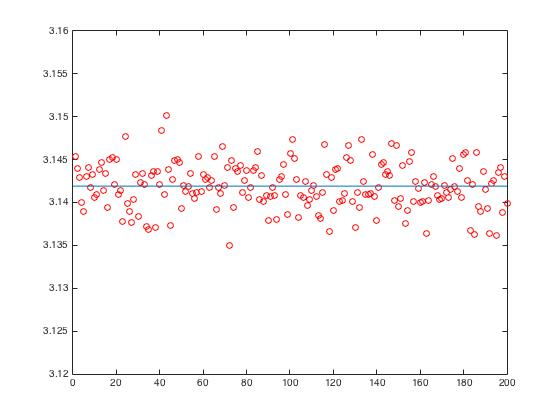
\includegraphics[width=9cm]{direkt200.jpg}
\caption{ Ergebnisse von 200 Durchl"aufen}
\end{figure}

\end{enumerate}